\xpartbox{Face Detection}

\begin{xpsectionbox}{Description}{}

Face detection determines the location and the size of a human face in an arbitrary digital image using:

\begin{minipage}{0.4\linewidth}

\begin{itemize}
	  \item low-level image features (Haar, LBP\footnote{T. Ojala, M. Pietikäinen, and D. Harwood, Performance evaluation of texture measures with classification based on Kullback discrimination of distributions, ICPR, 1994})
	  \item high-level facial landmarks (eye(s), nose, mouth, ear(s), chin, etc.)
	  \item skin color	
\end{itemize}
\end{minipage}
\begin{minipage}{0.6\linewidth}

\begin{center}
%			%\hspace{-5cm}
%			\vspace{-1cm}
			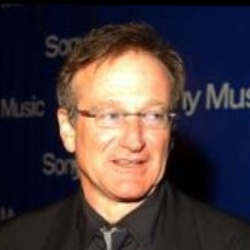
\includegraphics[height=0.25\linewidth]{images/RW_orig}
			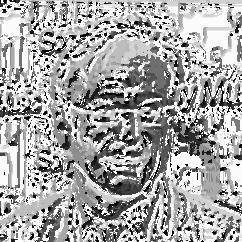
\includegraphics[height=0.25\linewidth]{images/RW_lbp}
			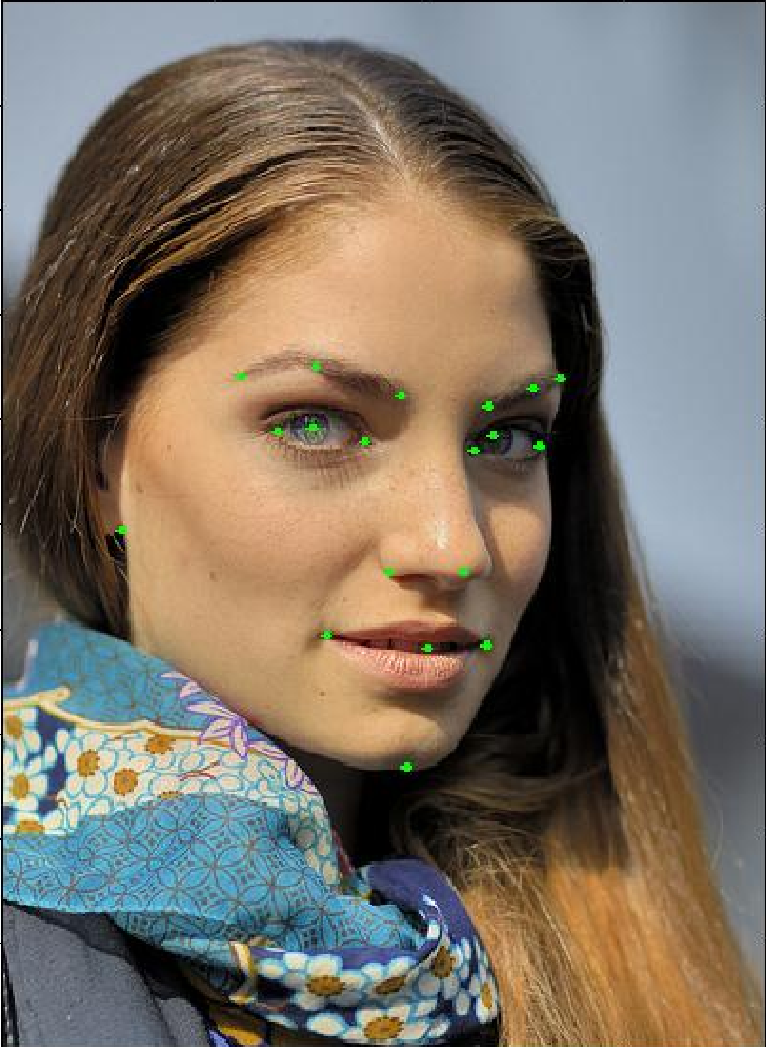
\includegraphics[height=0.25\linewidth]{images/facial_landmarks}
			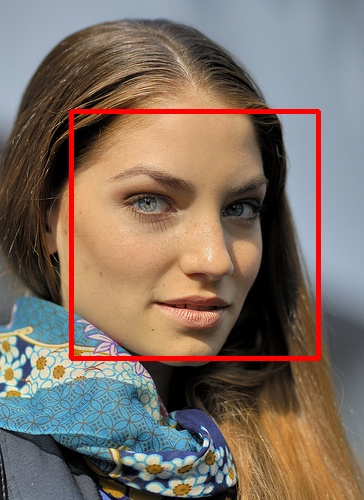
\includegraphics[height=0.25\linewidth]{images/image00168}
\end{center}

\end{minipage}
\end{xpsectionbox}

%\begin{xpsectionbox}{Challenges}{}
%
%\begin{minipage}{0.4\linewidth}
%\begin{itemize}
%	  \item low-quality images
%	  \item various lighting conditions
%	  \item frontal vs. profile faces
%	  \item various skin colors
%	  \item occlusions, facial hair, glasses, hat, etc.
%\end{itemize}
%\end{minipage}
%\begin{minipage}{0.6\linewidth}
%\begin{center}
%			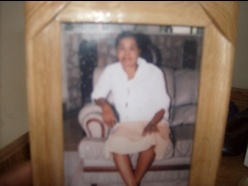
\includegraphics[height=0.25\linewidth]{images/PL_low_quality}
%			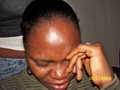
\includegraphics[height=0.25\linewidth]{images/HEPL_occlusion}
%			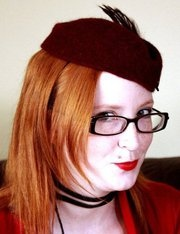
\includegraphics[height=0.25\linewidth]{images/HEPL_spectacles_hat}
%\end{center}
%\end{minipage}
%
%\end{xpsectionbox}

\xpartbox{Solution}

%--------------------------------------------------------------------------------------------------------------------
\begin{xpsectionbox}{}{}


\begin{minipage}{0.5\linewidth}

{\vspace*{0.2cm}\noindent\hspace*{0.2cm}{\bf\Titlesize Method}\newline}{\vspace{-0.75cm}}

\begin{itemize}
	  \item Haar like features  
	  \item moving window technique
	  \item Ada boost classifier cascade (Viola-Jones\footnote{P. Viola and M. Jones, Rapid Object Detection using a Boosted Cascade of Simple Features, CVPR, 2001})
\end{itemize}
\begin{center}
			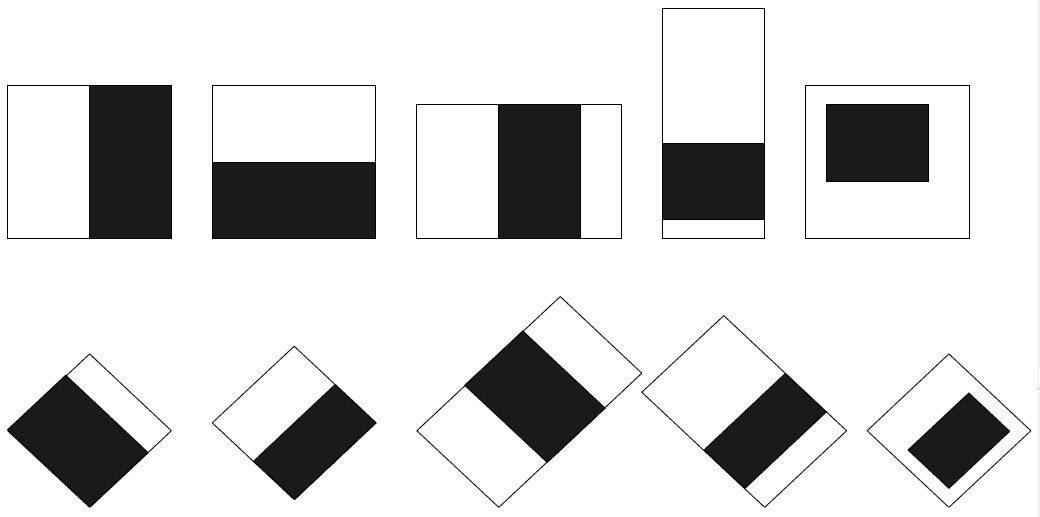
\includegraphics[height=0.25\linewidth]{images/Haar_features}
\end{center}

{\vspace*{0.2cm}\noindent\hspace*{0.2cm}{\bf\Titlesize Drawbacks}\newline}{\vspace{-0.75cm}}

\begin{itemize}
	  \item small size faces not detectable
	  \item lighting/occlusion deteriorates results 
\end{itemize}
\begin{center}
			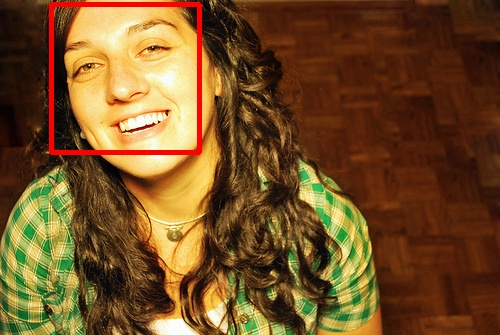
\includegraphics[height=0.2\linewidth]{images/image00613}
			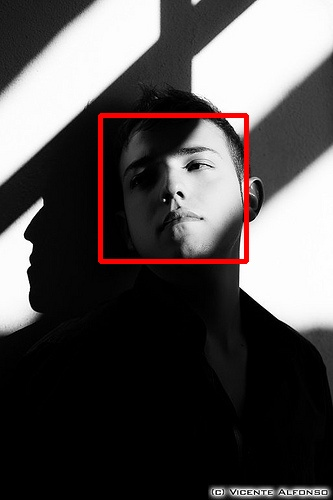
\includegraphics[height=0.2\linewidth]{images/image00571}
			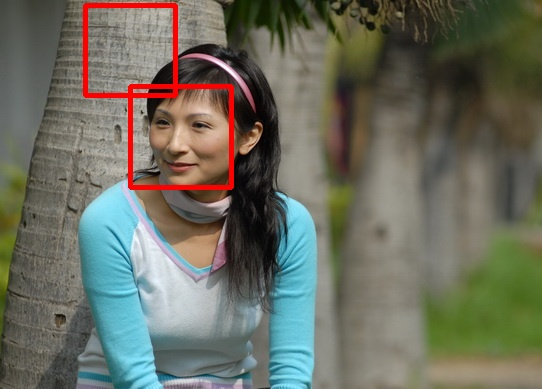
\includegraphics[height=0.2\linewidth]{images/image00210}
\end{center}

\end{minipage}
\begin{minipage}{0.5\linewidth}

\vspace{-2.5cm}
{\vspace*{0.2cm}\noindent\hspace*{0.2cm}{\bf\Titlesize Improvements}\newline}{\vspace{-0.75cm}}

\begin{itemize}
	  \item color information (skin) 
	  \item learning color models
	  \item extended color space + neural network
\end{itemize}
\begin{center}
			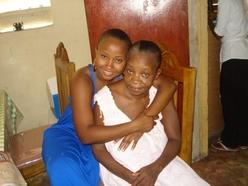
\includegraphics[height=0.16\linewidth]{images/Lena_RGB}
			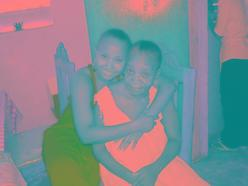
\includegraphics[height=0.16\linewidth]{images/Lena_LAB}
			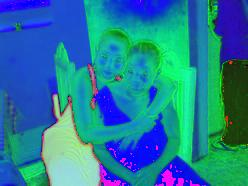
\includegraphics[height=0.16\linewidth]{images/Lena_HSV}
			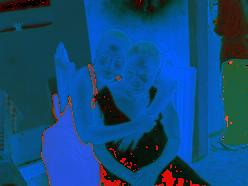
\includegraphics[height=0.16\linewidth]{images/Lena_LUV}
\end{center}

{\vspace*{0.2cm}\noindent\hspace*{0.2cm}{\bf\Titlesize Advantages}\newline}{\vspace{-0.75cm}}

\begin{itemize}
	  \item high precision skin detection(91\%)  
	  \item skin maps focus the face finding
	  \item enhance skin region intensities
\end{itemize}
\begin{center}
			
			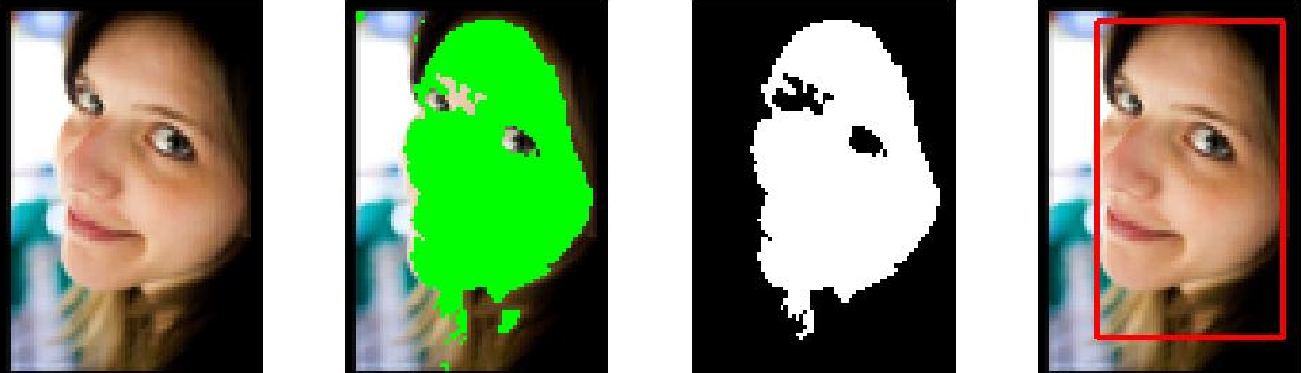
\includegraphics[height=0.2\linewidth]{images/skin_color_demo}
\end{center}
\end{minipage}
\end{xpsectionbox}

\xpartbox{Experiments}

\begin{xpsectionbox}{}{}
With no modifications, Viola-Jones face detector misses about half of the HEPL faces, and about 20\% of the missed ones are typically too small for matching purposes.

Accuracy results of our FaceFinder
\begin{itemize}
	\item HEPL-300: R=75\%, P=83\%, F=79\%
	\item HEPL-4K (noisy): F=53\%
	\item PL-700nd+skin: 46\% Recall boost with 22\% FP rate
\end{itemize}
The major factors hurting the accuracy are: Lighting=5.3\%; Quality=8.8\%; Occlusion=10.8\%; Color=0.6\%; Combination=9.5\%; Small Faces=20.8\%; Other=44.2\%.
\end{xpsectionbox}


%\xpartbox{Evaluation data}
%%--------------------------------------------------------------------------------------------------------------------
%\begin{xpsectionbox}{Data description}{}
%
%\begin{minipage}{0.4\linewidth}
%\begin{itemize}
%		\item $50$ Bangla city names (vocabulary)
%		\item $163$ writers
%	  \item $14,073$ city name samples
%	  \item $7,557$ samples for training (87 writers)
%	  \item $6,516$ samples for test (76 writers)
%	  \item data annotated on word level
%\end{itemize}
%\end{minipage}
%\nolinebreak
%\begin{minipage}{0.6\linewidth}
%		\begin{center}
%			%\hspace{-5cm}
%			\vspace{-1cm}
%			%\includegraphics[height=0.5\linewidth]{images/BanglawordSamples.pdf}\\%
%		\end{center}
%\end{minipage}
%\end{xpsectionbox}
%
%%--------------------------------------------------------------------------------------------------------------------
%
%
%%--------------------------------------------------------------------------------------------------------------------
%%\begin{xpsectionbox}{Network setup}{}
%%\begin{minipage}{0.7\linewidth}
%%\begin{itemize}
%%	  \item fully connected multi-layer perceptron
%%	  \item sigmoid transfer function
%%	  \item error back-propagation
%%	  \item $784-500-10$ topology
%%	  
%%\end{itemize}
%%\end{minipage}
%%\nolinebreak
%%	\begin{minipage}{0.3\linewidth}
%%		\begin{center}
%%			\hspace{-5cm}
%%			\vspace{1.5cm}
%%			\includegraphics[height=0.75\linewidth]{images/mlp.jpg}\\%
%%		\end{center}
%%	\end{minipage}
%%\end{xpsectionbox}
%%--------------------------------------------------------------------------------------------------------------------
%%--------------------------------------------------------------------------------------------------------------------
%%--------------------------------------------------------------------------------------------------------------------
%
%
%
%\xpartbox{Evaluation results}
%
%\begin{xpsectionbox}{Writer independent word recognition}{}
%
%{\bf Model details:}
% 
%\begin{itemize}
%		\item semi-continuous HMMs (ESMERALDA)
%	  \item Bakis topology
%	  \item codebook of $1$k Gaussians with diagonal covariance matrices
%	  \item 20 Baum-Welch training epochs
%\end{itemize}	
%
%\vspace{2cm}
%
%{\bf Recognition results achieved for differently structured writing models:}
%\vspace{1cm}
%
%		\begin{center}	
%    \begin{tabular}{l|r|r|r}
%	Writing Model	&	\multicolumn{2}{c|}{Complexity} &	Rec. Rate \\
%			&	units &	indep. states &	[\%] \\
%	\hline
%	\hline
%	holistic &		50 &	1,645 &	88.0	\\
%	combined characters &	93 &	876 &	88.5	\\
%	pseudo-characters &	52 &	286 &	91.0	\\
%	context-dependent &	293 &	362 (1,714) &	93.1	\\
%	\hline
%	\end{tabular}
%    \end{center}
%    %\caption{Recognition results achieved for differently structured writing models}
%    %\label{tab:results}
%%\end{table}
%
%\vspace{2cm}
%
%{\bf Comments:} 
%\begin{itemize}
%		\item holistic: each word is represented as a single entity
%	  \item combined-characters: modeling basic character, modifiers and combined characters
%	  \item pseudo-characters: modeling just basic character shapes and modifiers
%	  \item context-dependent: modeling pseudo characters and their left and right context
%\end{itemize}	
%\end{xpsectionbox}